\documentclass[12pt]{article}
\usepackage[UTF8]{ctex}
\usepackage[textwidth=450bp,vmargin=2.5cm]{geometry}%设置页边距
\setlength{\parskip}{0.5em}
\usepackage{array} %主要是增加列样式选项
\usepackage[dvipsnames]{xcolor}%颜色宏包
\usepackage{graphicx}%图片宏包
\usepackage{subfigure}%并排图片.
\usepackage{wrapfig}
\usepackage{amsmath}%公式宏包
\usepackage{threeparttable}%表格注释
\usepackage[T1]{fontenc}    %字体编码
\usepackage{newtxtext, newtxmath}  %两种使用Times New Roman 字体的方法
\usepackage{subfigure}%并排图片
\usepackage{float}
\usepackage{amssymb}%罗马数字\rmnum小写 \Rmnum大写
\makeatletter
\newcommand{\rmnum}[1]{\romannumeral #1}
\newcommand{\Rmnum}[1]{\expandafter\@slowromancap\romannumeral #1@}
\makeatother
%%%设置段落颜色
\usepackage{color}
%\definecolor{shadecolor}{named}{Gray}
\definecolor{shadecolor}{rgb}{0.5,0.5,0.5}
\usepackage{framed}
%%%设置页面颜色
\usepackage{xcolor}

\title{电动力学}
\author{SCAT}
\date{September 2023}

\begin{document}
\definecolor{backgroundcolor}{RGB}{60, 60, 60}
\pagecolor{backgroundcolor}
\maketitle
\color[RGB]{220,220,220}
\section{数学基础}
\begin{shaded}
$$
  \int_a^b f(x) dx
$$
\end{shaded}
\section{\textit{Maxwell} 方程组}
\subsection{真空中的\textit{Maxwell} 方程组}
真空中的\textit{Maxwell }方程组微分形式:
\begin{equation}
\left\{\begin{split}
   \nabla \cdot \Vec{E}&=\frac{\rho}{\varepsilon_0} \\
   \nabla \times \Vec{E}&=-\frac{\partial \Vec{B}}{\partial t}  \\
   \nabla \cdot \Vec{B}&=0  \\
   \nabla \times \Vec{B}&=\mu_0 \Vec{j}+\mu_0\varepsilon_0\frac{\partial \Vec{E}}{\partial t}  
\end{split}\right.
\label{x1}
\end{equation}
积分形式:
\begin{equation}
    \left\{\begin{split}
    \oint_S \Vec{E}\cdot \mathrm{d}\Vec{S}&=\int_V \frac{\rho}{\varepsilon_0} \mathrm{d}V \\
   \oint_l \Vec{E}\cdot\mathrm{d}\Vec{l}&=-\int_S \frac{\partial \Vec{B}}{\partial t}\cdot \mathrm{d}\Vec{S}  \\
   \oint_S \Vec{B}\cdot \Vec{S}&=0  \\
   \oint_l \Vec{B}\cdot \mathrm{d}\Vec{l}&=\mu_0 I +\mu_0\varepsilon_0\int_s \frac{\partial \Vec{E}}{\partial t}\cdot \mathrm{d}\Vec{S}
    \end{split}\right.
\end{equation}
其中$\Vec{j}\equiv \rho\Vec{v} $为电流密度:
\begin{equation}
\begin{split}
    \Vec{j}&=\frac{\Delta q}{\Delta t\Delta S}=\frac{\rho \Delta \Vec{V}}{\Delta t\Delta S}=\frac{\rho \Delta S\cdot \Vec{v}\Delta t}{\Delta t\Delta S}=\rho\Vec{v}\\
    I&=\int_S \Vec{j}\cdot \mathrm{d}\Vec{S}
\end{split}
\end{equation}

\textbf{连续性方程}:
\begin{equation}
    \nabla\cdot\Vec{j}+\frac{\partial}{\partial t}\rho=0
    \label{x2}
\end{equation}
推导过程:\\
      由电荷守恒可知:
      \begin{equation}
            \oint_S \Vec{j}\cdot \mathrm{d}\Vec{S}=-\frac{\mathrm{d}}{\mathrm{d}t}\int_V \rho \mathrm{d}V
      \end{equation}
        其中左边代表电荷流出量,右边代表电荷的减少量,由散度定理:
        \begin{equation}
            \int_V \nabla\cdot \Vec{j}\mathrm{d}V=-\int_V \frac{\partial}{\partial t}\rho \mathrm{d}V
        \end{equation}
        取相同的体积元积分,并把积分号去掉可得(\ref{x2})。
        
真空中电磁场以电磁波的形式传播:
\begin{equation}
    \nabla^2 \Vec{E}-\frac{1}{c^2}\frac{\partial^2 \Vec{E}}{\partial t^2}=0\label{x11}
\end{equation}
其中$c=\frac{1}{\sqrt{\mu_0\varepsilon_0}}$是光速(也就是电磁波在真空的传播速度),首先根据矢量矢量叉乘的性质$\Vec{a}\times (\Vec{b}\times\Vec{c})=\Vec{b}(\Vec{a}\cdot\Vec{c})-\Vec{c}(\Vec{a}\cdot\Vec{b})$有:
\begin{equation}
\nabla\times(\nabla\times\Vec{E})=\nabla(\nabla\cdot\Vec{E})-\nabla^2\Vec{E}
\end{equation}
根据上式和(\ref{x1})可知:
\begin{equation}
    \begin{split}
        \nabla^2\Vec{E}&=\nabla(\nabla\cdot\Vec{E})-\nabla\times(\nabla \times\Vec{E})\\
    &=\nabla(\frac{\rho}{\varepsilon_0})+\nabla\times(\frac{\partial }{\partial t}\Vec{B})\\
    &=\frac{\partial}{\partial t}(\nabla\times \Vec{B})\\
    &=\mu_0\varepsilon_0\frac{\partial^2 \Vec{E}}{\partial t^2}
    \end{split}
\end{equation}
其中$\frac{\rho}{\varepsilon_0}$为常量,$\nabla$作用在其身上为0,第三行是$\nabla$与时间偏导运算进行交换。
\subsection{\textit{Maxwell}方程组的简要推导}
\subsubsection{方程\Rmnum{1}:电场的散度}
由库仑定律:
\begin{equation}
    \Vec{E}\cdot\mathrm{d}\Vec{S}=\frac{Q}{4\pi\varepsilon_0r^2}\cos{\theta}\mathrm{d}S
\end{equation}
根据立体角的定义$\mathrm{d}\Omega=\frac{\cos{\theta}}{r^2}\mathrm{d}S$,可得到高斯定理:
\begin{equation}
\begin{split}
    \oint_S \Vec{E}\cdot\mathrm{d}\Vec{S}&=\frac{Q}{4\pi\varepsilon_0}\oint\mathrm{d}\Omega=Q/\varepsilon_0\\
    \Rightarrow \oint_S \Vec{E}\cdot \mathrm{d}\Vec{S}&=\int_V \frac{\rho(\Vec{r'})}{\varepsilon_0}\mathrm{d}V
\end{split}
\end{equation}
根据散度定理:
\begin{equation}
    \int_V \nabla\cdot\Vec{E}\mathrm{d}V=\int_V \frac{\rho(\Vec{x'})}{\varepsilon_0}\mathrm{d}V
\end{equation}
取相同的积分体积元,即可得到:
\begin{equation}
    \nabla\cdot\Vec{E}(\Vec{x})=\frac{\rho(\Vec{x})}{\varepsilon_0}
\end{equation}
\subsubsection{方程\Rmnum{2}:电场的旋度}
在无磁场的情况下,电场只能由电荷产生:
\begin{equation}
    \oint_l \Vec{E}\cdot \mathrm{d}\Vec{l}=\frac{Q}{4\pi \varepsilon_0}\oint \frac{\Vec{r}}{r^3}\cdot\mathrm{d}\Vec{l}=\frac{Q}{4\pi\varepsilon_0}\oint_l \frac{1}{r^2} \mathrm{d}r=0
\end{equation}
可见,电荷的纯在对于电场的旋度不起作用,我们考虑磁场的作用,由电磁感应定律:
\begin{equation}
    \mathcal{E}=-\frac{\mathrm{d}\Phi}{\mathrm{d}t}=-\frac{\mathrm{d}}{\mathrm{d}t}\int_S \Vec{B}\cdot\mathrm{d}\Vec{S}
\end{equation}
其中$\mathcal{E}$为感应电动势:
\begin{equation}
    \mathcal{E}=\oint_l \Vec{E}\mathrm{d}\Vec{l} 
\end{equation}
那么在随时间变化的磁场中有:
\begin{equation}
    \oint_l \Vec{E}\cdot\mathrm{d}\Vec{l}=-\frac{\mathrm{d}}{\mathrm{d}t}\int_S \Vec{B}\cdot\mathrm{d}\Vec{S}
\end{equation}
由散度定理,并交换右边项对时间求导与面积分的次序:
\begin{equation}
    \int_S \nabla\times \Vec{E}\cdot\mathrm{d}\Vec{S}=\int_S -\frac{\partial }{\partial t}\Vec{B}\cdot\mathrm{d}\Vec{S}
\end{equation}
取相同的面积元,去掉积分号,得到:
\begin{equation}
    \nabla\times \Vec{E}=-\frac{\partial}{\partial t}\Vec{B}
\end{equation}
\subsubsection{方程\Rmnum{3}:磁场的散度}
由毕奥-萨伐尔定律:
\begin{equation}
    \Vec{B}(\Vec{x})=\frac{\mu_0}{4\pi}\int_V \frac{\Vec{j}(\Vec{x'})\times \Vec{r}}{r^3}\mathrm{d}V
\end{equation}
定义矢势:
\begin{equation}
   \Vec{A}=\frac{\mu_0}{4\pi}\int_V \frac{\Vec{j}(\Vec{x'})}{r}\mathrm{d}V 
   \label{x3}
\end{equation}
可以计算出$\Vec{B}(\Vec{x})=\nabla\times \Vec{A}$,注意$\nabla$是对场点$\Vec{x}$的作用,对源点$\Vec{x'}$无作用,所以:
\begin{equation}
\begin{split}
     \nabla\times\Vec{A}&=\nabla\times\frac{\mu_0}{4\pi}\int_V
\frac{\Vec{j}(\Vec{x'})}{r}\mathrm{d}V\\ 
    &=\frac{\mu_0}{4\pi}\int_V \nabla\times \frac{\Vec{j}(\Vec{x'})}{r}\mathrm{d}V\\
    &=-\frac{\mu_0}{4\pi}\int_V \Vec{j}(\Vec{x'})\times\nabla(\frac{1}{r})\mathrm{d}V\\
    &=\frac{\mu_0}{4\pi}\int_V \frac{\Vec{j}(\Vec{x'})\times\Vec{r}}{r^3}\mathrm{d}V=\Vec{B}(\Vec{x})
\end{split}
\end{equation}
因此磁场的散度为:
\begin{equation}
    \nabla\cdot\Vec{B}(\Vec{x})=\nabla\cdot\nabla\times\Vec{A}=0
\end{equation}
\subsubsection{方程\Rmnum{4}:磁场的旋度}\footnote{这个推导没有使用位移电流假设。}
利用矢势可以把磁场的旋度化为:
\begin{equation}
\nabla\times\Vec{B}=\nabla\times(\nabla\times\Vec{A})=\nabla(\nabla\cdot\Vec{A})-\nabla^2\Vec{A}
\label{x4}
\end{equation}
先计算第一项中的$\nabla\cdot\Vec{A}$,根据矢势的定义(\ref{x3}):
\begin{equation}
    \nabla\cdot\Vec{A}=\nabla\cdot\frac{\mu_0}{4\pi}\int_V \frac{\Vec{j}(\Vec{x'})}{r}\mathrm{d}V=\frac{\mu_0}{4\pi}\int_V \Vec{j}(\Vec{x'})\cdot\nabla(\frac{1}{r})\mathrm{d}V
\end{equation}
这里仍然需要注意的是$\nabla$只作用在$\Vec{x}$上,定义$\nabla'$只作用在$\Vec{x'}$上,由$\Vec{r}=\Vec{x}-\Vec{x'}$,所以$\nabla f(\Vec{r})=-\nabla' f(\Vec{r}) $,由此可得:
\begin{equation}
\begin{split}
   \nabla\cdot\Vec{A} 
   &=-\frac{\mu_0}{4\pi}\int_V \nabla'(\frac{1}{r})\cdot\Vec{j}(\Vec{x'})\mathrm{d}V\\
   &=-\frac{\mu_0}{4\pi}\int_V [\nabla'\cdot \frac{\Vec{j}(\Vec{x'})}{r}-\frac{1}{r}\nabla'\cdot\Vec{j}(\Vec{x'})]\mathrm{d}V  
\end{split}
\end{equation}
先看第一项的积分:
\begin{equation}
    -\frac{\mu_0}{4\pi}\int_V \nabla'\cdot\frac{\Vec{j}(\Vec{x'})}{r}\mathrm{d}V=-\frac{\mu_0}{4\pi}\oint_S \frac{\Vec{j}(\Vec{x'})}{r}\cdot\mathrm{d}\Vec{S}=0
\end{equation}
由于电流分布在有限的区域,当$\Vec{x'}\to \infty$时,也就是无穷远处的边界电流密度一定为0,所以这一项的积分为0。\\
那么$\nabla\cdot\Vec{A}$只有第二项起作用,所以(\ref{x4})中第一项为:
\begin{equation}
\begin{split}
    \nabla(\nabla\cdot\Vec{A})&=-\frac{\mu_0}{4\pi}\frac{\partial}{\partial t}\int_V \nabla[\frac{\rho(\Vec{{x'}})}{r}]\mathrm{d}V\\
    &=-\frac{\mu_0}{4\pi}\frac{\partial}{\partial t}\int_V \rho(\Vec{x'})\nabla(\frac{1}{r})\mathrm{d}V\\
    &=\frac{\mu_0}{4\pi}\frac{\partial}{\partial t}\int_V \frac{\rho(\Vec{x'})}{r^3}\Vec{r}\mathrm{d}V\\
    \end{split}
    \label{x5}
\end{equation}
其中第三行用到了$\nabla\frac{1}{r}=-\frac{\Vec{r}}{r^3}$,回忆场强的定义:
\begin{equation}
    \Vec{E}(\Vec{x})=\int_V \frac{\rho(\Vec{x'})}{4\pi\varepsilon_0}\frac{\Vec{r}}{r^3}\mathrm{d}V
\end{equation}
那么(\ref{x5})可以化为:
\begin{equation}
\nabla(\nabla\cdot\Vec{A})=\mu_0\varepsilon_0\frac{\partial}{\partial t}\Vec{E}(\Vec{x})
\end{equation}
我们发现这一项其实就是\textit{Maxwell}假设的位移电流,这里我们通过矢势的定义直接计算出了这一项。

接下来计算$\nabla^2\Vec{A}$,这里计算过程中需要注意的是$\nabla^2\frac{1}{r}=-4\pi\delta(r)$:
\begin{equation}
    \begin{split}
        \nabla^2\Vec{A}&=\frac{\mu_0}{4\pi}\int_V \nabla^2\frac{\Vec{j}(\Vec{x'})}{r}\mathrm{d}V\\
        &=-\frac{\mu_0}{4\pi}\int_V \Vec{j}(\Vec{x'})\nabla^2\frac{1}{r}\mathrm{d}V\\
        &=-\frac{\mu_0}{4\pi}\int_V \Vec{j}(\Vec{x'})\cdot4\pi\delta(r)\mathrm{d}V\\
        &=-\mu_0 \Vec{j}(\Vec{x})
    \end{split}
\end{equation}
那么最终可以计算出$\Vec{B}$的旋度为:
\begin{equation}
    \nabla\times\Vec{B}=\nabla(\nabla\cdot\Vec{A})-\nabla^2\Vec{A}=\mu_0\varepsilon_0 \frac{\partial}{\partial t}\Vec{E}+\mu_0 \Vec{j}(\Vec{x})
\end{equation}
\subsection{有介质纯在的\textit{Maxwell}方程组及边值条件}
\subsubsection{介质中的\textit{Maxwell}方程组}
介质中的Mawxwell方程组微分形式:
\begin{equation}
    \left\{
    \begin{split}
        \nabla\cdot\Vec{D}&=\rho_f\\
        \nabla\times\Vec{E}&=-\frac{\partial}{\partial t}\Vec{B}\\
        \nabla\cdot\Vec{H}&=0\\
        \nabla\times\Vec{H}&=\Vec{j_f}+\frac{\partial}{\partial t}\Vec{D}
    \end{split}\right.
    \label{x7}
\end{equation}
积分形式:
\begin{equation}\left\{
    \begin{split}
        \int_S \Vec{D}\cdot\mathrm{d}\Vec{S}&=Q_f\\
        \oint_l \Vec{E}\cdot\mathrm{d}\Vec{l}&=-\frac{\mathrm{d}}{\mathrm{d}t}\int_S \Vec{B}\cdot\Vec{S}\\
        \int_S \Vec{H}\cdot\mathrm{d}\Vec{S}&=0\\
        \oint_l \Vec{H}\cdot\mathrm{d}\Vec{l}&=I_f+\frac{\mathrm{d}}{\mathrm{d}t}\int_S \Vec{D}\cdot\mathrm{d}\Vec{S}
    \end{split}\right.
    \label{x6}
\end{equation}
对于(线性)介质有本构关系\footnote{其中只有线性介质满足$\varepsilon_r=1+\chi_e, \mu_r=1+\chi_M$。}:
\begin{equation}
    \left\{\begin{split}
&\Vec{D}=\varepsilon\Vec{E}\quad\quad&\varepsilon=\varepsilon_r\varepsilon_0=(1+\chi_e)\varepsilon_0\\
&\Vec{H}=\frac{1}{\mu}\Vec{B}\quad\quad&\mu=\mu_r\mu_0=(1+\chi_M)\mu_0
    \end{split}\right.
\end{equation}
其中$\varepsilon_r$为相对介电常数,$\mu_r$为相对磁导率。\\
定义极化强度和磁化强度\footnote{都是宏观小微观大,尤其指这里的$\Delta V$。}:
\begin{equation}
    \Vec{P}=\frac{\sum_i \Vec{P}}{\Delta V}\quad\quad\Vec{M}=\frac{\sum_i \Vec{m_i}}{\Delta V}
\end{equation}
这里的$\Vec{p}\equiv q\Vec{l}$为电偶极矩,$\Vec{m}=i\Vec{a}$为分子电流的磁矩。对于线性介质,极化强度和磁化强度满足:
\begin{equation}
    \left\{\begin{split}
        \Vec{P}(\Vec{x},t)&=\varepsilon_0\chi_e\Vec{E}(\Vec{x},t)\\
        \Vec{M}(\Vec{x},t)&=\frac{1}{\mu_0}\frac{\chi_M}{1+\chi_M}\Vec{B}(\Vec{x},t)
    \end{split}\right.
\end{equation}
\subsubsection{电磁场的边值条件}
\begin{wrapfigure}[8]{r}{10em}
\begin{center}
	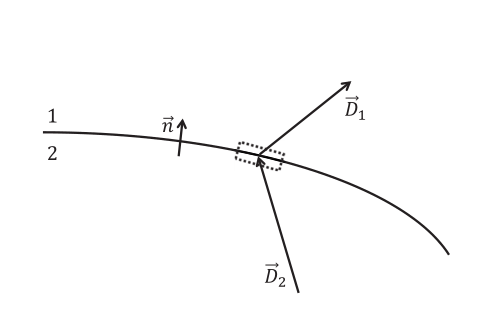
\includegraphics[width=2in]{F1.png}
	\label{F1}
\end{center}
\caption{电场界面}
\end{wrapfigure}
\footnote{未完待续。。。}在界面上,由于介质的突变导致\textit{Maxwell}方程组的微分形式不再适用,但是积分形式仍可以使用,先看第一条方程(\ref{x6}):
\begin{equation}
    \oint_S \Vec{D}\cdot\mathrm{d}\Vec{S}=\int_V \rho_f\mathrm{d}V
\end{equation}
当我们取界面上非常薄的一面时,也就是沿$\Vec{n}$方向上的长度趋近于0,设界面上电荷面密度为$\sigma_f\equiv \frac{q_f}{\Delta S} $,则有:
\begin{equation}\left\{
\begin{split}
&\oint_S \Vec{D}\cdot\mathrm{d}\Vec{S}=\Vec{D}_1\Delta S\cdot \Vec{n}-\Vec{D}_2\Delta S\cdot\Vec{n} = q_f
 \\ &\Rightarrow   (\Vec{D}_1-\Vec{D}_2)\cdot\Vec{n}=\sigma_f
\end{split}\right.
\end{equation}
所以当界面存在$\sigma_f$时,$\Vec{D}$场法向分量发生突变。%\begin{wrapfigure}[8]{r}{10em}
%\begin{center}
%	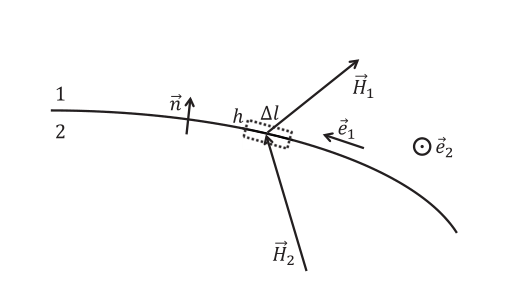
\includegraphics[width=2in]{F2.png}
%	\label{F2}
%\end{center}
%\end{wrapfigure}
在磁场中,如右图所示,$\Vec{e}_1, \Vec{e}_2$为界面上2个互相垂直的单位矢量,$\Vec{e}_1, \Vec{e}_2, \Vec{n}$呈右手螺旋:
\begin{equation}
\left\{\begin{split}
    \Vec{n}&=\Vec{e}_1\times \Vec{e}_2\\
    \Vec{e}_1&=\Vec{e}_2\times \Vec{n}\\
    \Vec{e}_2&=\Vec{n}\times \Vec{e}_1
    \end{split}\right.
\end{equation}
类似的,对于磁场由于磁场无源$(\nabla \cdot \Vec{H}=0)$可知:
\begin{equation}
    \oint_S \Vec{H}\cdot \mathrm{d}\Vec{S}=(\Vec{H}_1-\Vec{H}_2)\cdot \Vec{n}=0
\end{equation}
所以在有介质情况下$\Vec{H}$场的法向分量仍然守恒。\\
再讨论电场的情况,根据(\ref{x6})第二条方程计算,取边界围道法向($\Vec{n}$)长度趋于0,切向($\Vec{\tau}$)长度为$l$,则有:
\begin{equation}
\left\{\begin{split}
    &\oint_l \Vec{E}\mathrm{d}\Vec{l}=(\Vec{E}_1-\Vec{E}_2)\cdot l\Vec{\tau}=-\frac{\mathrm{d}}{\mathrm{d}t}\int_S \Vec{B}\cdot\mathrm{d}\Vec{S}=0\\
&\Rightarrow (\Vec{E}_1-\Vec{E}_2)\cdot \Vec{\tau}=0
\end{split}\right.
\end{equation}
所以$\Vec{E}$场切向分量守恒(连续)。\\
最后看磁场的切向分量情况,同样利用环路积分:
\begin{equation}
    \oint \Vec{H}\cdot\mathrm{d}\Vec{l}=\int_S (\Vec{j}_f+\frac{\partial}{\partial t}\Vec{D})\cdot\Vec{S}
\end{equation}
可以得到:
\begin{equation}
    \Vec{n}\times (\Vec{H}_1-\Vec{H}_2)=\Vec{\alpha}_f
\end{equation}
其中$\Vec{\alpha}_f$是面电流,也就是说存在$\Vec{\alpha}_f$时$\Vec{H}$场存在切向分量突变。
\subsection{电磁场的能量和能流}
\textbf{玻印廷矢量}:
\begin{equation}
    \Vec{S}=\Vec{E}\times\Vec{H}
    \label{x8}
\end{equation}
\textbf{电磁场能量密度}:
\begin{equation}
    w=\frac{1}{2}(\varepsilon_0 \Vec{E}^2+\frac{1}{\mu_0}\Vec{B}^2)
    \label{x9}
\end{equation}
下面是推导过程:由洛伦兹力力密度:
\begin{equation}
    \Vec{f}_l =\rho\Vec{E}+\Vec{j}\times\Vec{B}
\end{equation}
其中$\rho$是电荷密度,$\Vec{j}\equiv \rho\Vec{v}$是电流密度。由此可以计算出电磁场对电荷系统做功功率:
\begin{equation}
\begin{split}
    \int_V \Vec{f}\cdot\Vec{v}\mathrm{d}V&=\int_V \rho\Vec{E}\cdot \Vec{v}+\rho\Vec{v}\times\Vec{B}\cdot\Vec{v}\;\mathrm{d}V\\
    &=\int_V \Vec{E}\cdot \Vec{j}\mathrm{d}V
\end{split}
\end{equation}
由(\ref{x7})中第4条方程:
\begin{equation}
    \Vec{j}=\nabla\times\Vec{H}-\frac{\partial}{\partial t}\Vec{D}
\end{equation}
那么电磁场做功功率密度为:
\begin{equation}
\begin{split}
    \Vec{E}\cdot\Vec{j}&=\Vec{E}\cdot(\nabla\times\Vec{H})-\varepsilon_0\Vec{E}\frac{\partial}{\partial t}\Vec{E}\\
   &=-\nabla\cdot(\Vec{E}\times \Vec{H})+\Vec{H}\cdot(\nabla\times\Vec{E})-\frac{\varepsilon_0}{2}\frac{\partial}{\partial t }\Vec{E}^2
    \\
    &=-\nabla \cdot (\Vec{E}\times \Vec{H})-\frac{1}{2}\frac{\partial }{\partial t}(\frac{1}{\mu_0}\Vec{B}^2+\varepsilon_0\Vec{E}^2)
    \end{split}
\end{equation}
其中第三个等号用到了\textit{Maxwell}方程中的($\nabla\times\Vec{E}=-\frac{\partial}{\partial t}\Vec{B}$),那么也就是说电荷系统机械能($E_m$)增加的功率为\footnote{电荷系统机械能增加等于电磁场做功。}:
\begin{equation}
\begin{split}
    \frac{\mathrm{d} E_m}{\mathrm{d}t}&=\int_V \Vec{E}\cdot\Vec{j}\mathrm{d}V\\
    &=-\int_V[\nabla \cdot (\Vec{E}\times \Vec{H})+\frac{1}{2}\frac{\partial }{\partial t}(\frac{1}{\mu_0}\Vec{B}^2+\varepsilon_0\Vec{E}^2)]\mathrm{d}V\\
    &=-\oint_S \Vec{E}\times\Vec{H}\cdot\mathrm{d}S-\frac{1}{2}\frac{\partial}{\partial t}\int_V (\frac{1}{\mu_0}\Vec{B}^2+\varepsilon_0\Vec{E}^2)\mathrm{d}V
    \end{split}
\end{equation}
利用开头提到的定义(\ref{x8},\ref{x9}):
\begin{equation}
    \left\{\begin{split}
        &\frac{\mathrm{d}}{\mathrm{d}t}E_m=-\oint_S \Vec{S}_p\cdot\mathrm{d}\Vec{S}-\int_V w\mathrm{d}V\\
        &\Rightarrow \frac{\mathrm{d}}{\mathrm{d}t}[E_m+\int_V w\mathrm{d}V]=-\oint_S \Vec{S}_p\cdot\mathrm{d}\Vec{S}
    \end{split}\right.
\end{equation}
这里的物理图像实际就是能量守恒,左边是总能量的变化率,也就是机械能和电磁场能量的总变化率,也就是说$w$就是电磁场能量密度,右边是能量流,也就表明当$\Vec{S}_p$为正时,系统能量减少,也就是有能量流出系统,说明波印廷矢量$\Vec{S}_p$就是能量流密度\footnote{流出为正,流入为负,类比电流。}。\\
当区域为全空间时,没有能量从无穷远处流入流出,$\Vec{S}_p=0$:
\begin{equation}
    \left\{\begin{split}
       &\frac{\mathrm{d}}{\mathrm{d}t}[E_m+\int_V w\mathrm{d}V]=0\\
       &\Rightarrow E_m+\int_V w\mathrm{d}V=Const
    \end{split}\right.
\end{equation}
这表明无穷大界面机械能和电磁场能量的总能量守恒,这是显而易见的,因为电荷和电流总是分布在有限区域内,也就是电磁场总是存在于有限区域,由此当边界无穷大时电磁场能量与机械能之和不随时间变化。\\
当空间无源时,也就是不纯在电荷系统,也就没有机械能变化($\frac{\mathrm{d}}{\mathrm{d}t}E_m=0$):
\begin{equation}
\left\{\begin{split}
    \int_V \frac{\partial}{\partial t} w\mathrm{d}V+\oint_S \Vec{S}_p\cdot\mathrm{d}\Vec{S}&=0\\
    \frac{\partial}{\partial t}w+\nabla\cdot\Vec{S}_p&=0
\end{split}\right.
\end{equation}
这和连续性方程(\ref{x2})形式一样,物理意义就是无源场电磁场能量守恒\footnote{机械能一直不变了。}。

\section{电磁波的传播}
\subsection{平面电磁波}
\subsubsection{波动方程}
真空中$\Vec{E}$和$\Vec{B}$的波动方程(\ref{x11}):
\begin{equation}
    \left\{
    \begin{split}
        &\nabla^2 \Vec{E}-\frac{1}{c^2}\frac{\partial^2\Vec{E}}{\partial t^2}=0\\
        &\nabla^2 \Vec{B}-\frac{1}{c^2}\frac{\partial^2\Vec{B}}{\partial t^2}=0
    \end{split}\right.
    \label{x10}
\end{equation}
其中光速$c^2\equiv 1/\varepsilon_0\mu_0$。由真空中的\textit{Maxwell}\textit{'s Equation}(\ref{x1}),及本构关系:
\begin{equation}\left\{
    \begin{split}
        &\Vec{D}=\varepsilon_0 \Vec{E}\\
        &\Vec{B}=\mu_0 \Vec{H}
    \end{split}\right.
\end{equation}
由:
\begin{equation}
    \nabla\times(\nabla\times\Vec{E})=\nabla\times(-\frac{\partial\Vec{B}}{\partial t})=-\mu_0\varepsilon_0\frac{\partial^2 \Vec{E}}{\partial t^2}
\end{equation}
同时由$\Vec{A}\times(\Vec{B}\times\Vec{C})=(\Vec{A}\cdot\Vec{C})\Vec{B}-(\Vec{A}\cdot\Vec{B})\Vec{C}$可得:
\begin{equation}
\nabla\times(\nabla\times\Vec{E})=\nabla(\nabla\cdot\Vec{E})-\nabla^2\Vec{E}=-\nabla^2\Vec{E}
\end{equation}
这样即可得到(\ref{x10})中$\vec{E}$的方程,类似可以得到$\Vec{B}$的方程。\\
对于线性介质一般有色散关系:
\begin{equation}
    \left\{
    \begin{split}
        &\Vec{D}(\omega)=\varepsilon(\omega)\Vec{E}(\omega)\\
        &\Vec{B}(\omega)=\mu(\omega)\Vec{H}(\omega)
    \end{split}\right.
\end{equation}
对于一般介质得不到$\vec{E}$和$\Vec{B}$的波动方程,但是如果入射的是单色电磁波(固定的$\omega$)那么仍然有($\ref{x10}$),只需把光速$c$改为在该介质的波速$v=1/\sqrt{\varepsilon(\omega)\mu(\omega)}$。
\subsubsection{时谐电磁波}
对于频率一定的电磁波,有:\footnote{后面将默认$\Vec{E}=\Vec{E}'(\Vec{r}),\Vec{B}=\Vec{B}'(\Vec{r})$}
\begin{equation}
    \left\{\begin{split}
        &\Vec{E}(\Vec{r},t)=\Vec{E}'(\Vec{r})\mathrm{e}^{-i\omega t}\\
        &\Vec{B}(\Vec{r},t)=\Vec{B}'(\Vec{r})\mathrm{e}^{-i\omega t}
    \end{split}\right.
\end{equation}
设$\Vec{E},\;\Vec{B}$的空间分量和时间分量相互独立,则有:\footnote{因为时间因子在$E(\Vec{r},t)$和$\Vec{B}(\Vec{r},t)$中解的形式一样,故这里不作区分。}
\begin{equation}
    \left\{\begin{split}
        &\Vec{E}(\Vec{r},t)=\Vec{E}'(\Vec{r})T(t)\\
        &\Vec{B}(\Vec{r},t)=\Vec{B}'(\Vec{r})T(t)
    \end{split}\right.
    \label{x12}
\end{equation}
对于一般线性介质,以单色波射入,满足波动方程:
\begin{equation}
    \left\{
    \begin{split}
        &\nabla^2\Vec{E}(\Vec{r},t)-\frac{1}{v^2}\frac{\partial^2}{\partial^2}\Vec{E}(\Vec{r},t)=0\\
        &\nabla^2\Vec{B}(\Vec{r},t)-\frac{1}{v^2}\frac{\partial^2}{\partial^2}\Vec{B}(\Vec{r},t)=0
    \end{split}\right.
\end{equation}
其中$u=1/\sqrt{\mu\varepsilon}=c/\sqrt{\mu_r\varepsilon_r}$为介质中电磁波的波速,可以看出折射率:
\begin{equation}
    n\equiv \sqrt{\mu_r\varepsilon_r}
\end{equation}
回到波动方程,利用分离变量法,把(\ref{x12})带入波动方程中:
\begin{equation}
    \left\{\begin{split}
       & \frac{\nabla^2 \Vec{E}}{\Vec{E}}=\frac{1}{v^2}\frac{\partial^2 T/\partial t^2}{T}=-\frac{\omega^2}{v^2}=-k^2\\
       & \frac{\nabla^2 \Vec{B}}{\Vec{B}}=\frac{1}{v^2}\frac{\partial^2 T/\partial t^2}{T}=-\frac{\omega^2}{v^2}=-k^2
    \end{split}\right.
\end{equation}
可以解得:\footnote{工科物理好像用到是$\mathrm{e}^{i\omega t}$,物理人这里和那边差个负号。}
\begin{equation}
    T(t)=\mathrm{e}^{-i\omega t}
\end{equation}
对于空间部分,有:
\begin{equation}\left\{
    \begin{split}
        &\nabla^2\Vec{E}+k^2\Vec{E}=0\\
        &\nabla^2\Vec{B}+k^2\Vec{B}=0
    \end{split}\right.
    \label{x13}
\end{equation}

\subsubsection{平面电磁波}
在$\omega$一定的情况下,\textbf{绝缘介质}中的\textit{Maxwell}方程组可以化为:
\begin{equation}
    \left\{\begin{split}
        &\nabla^2 \Vec{E}+k^2\Vec{E}=0\\
         &\nabla\cdot\Vec{E}=0\Rightarrow \Vec{k}\cdot\Vec{E}=0\\
         &\Vec{B}=-\frac{i}{\omega}\nabla\times\Vec{E}=\frac{\Vec{k}}{\omega}\times\Vec{E}   
    \end{split}\right.
\end{equation}
或:
\begin{equation}
    \left\{\begin{split}
        &\nabla^2 \Vec{B}+k^2\Vec{B}=0\\
         &\nabla\cdot\Vec{B}=0\Rightarrow \Vec{k}\cdot\Vec{B}=0\\
         &\Vec{E}=\frac{i}{\omega\mu\varepsilon}\nabla\times\Vec{B}=-\frac{\Vec{k}}{\omega\mu\varepsilon}\times\Vec{B} =\frac{1}{v}\Vec{E}\times \vec{e}_k  
    \end{split}\right.
\end{equation}











\end{document}
